%\input{Preambulum}

\begin{figure}[t!]
\centering

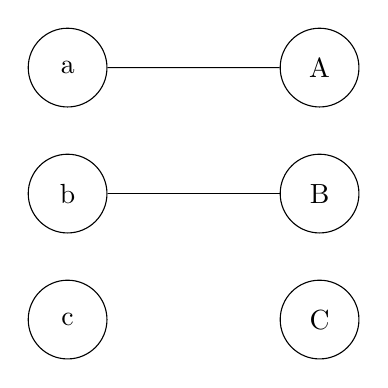
\begin{tikzpicture}[scale=0.8, auto=center]
\tikzstyle{every node}=[draw,shape=circle];
  \node[minimum size=1cm] (n1) at (0,4) {a};
  \node[minimum size=1cm] (n2) at (0,2) {b};
  \node[minimum size=1cm] (n3) at (0,0) {c};
  \node[minimum size=1cm] (n4) at (4,4) {A};
  \node[minimum size=1cm] (n5) at (4,2) {B};
  \node[minimum size=1cm] (n6) at (4,0) {C};

  \foreach \from/\to in {n1/n4,n2/n5}
    \draw (\from) -- (\to);
\end{tikzpicture}

\captionsetup{justification=centerfirst}
\caption{The only balanced bipartite graph up to six nodes where unfairness emerges \\ \vspace{0.2cm}
\footnotesize{\emph{Note}: Solid lines indicate the type constraints.}}
\label{Fig4}
\end{figure}

%\end{document}